\section{System Architecture}
\label{sec:systemarch}

% This was corrected in my version... (Joir-dan performing diff 2010-06-30)
This section presents ontology and corpora, query processing, ranking queries, and query executing.

\subsection{Using Ontology and Corpora} 
\label{sec:ontology_corpora}

Morpheus uses an ontology that contains classes of a particular realm of interest. Each leaf node in the ontology is associated with a corpus of words belonging to a class.  For example, we have constructed a vehicular ontology containing classes relevant to the vehicular realm. This ontology provides a structure for reference in the following sections.

%% Need ontology paragraph


Morpheus references the DBpedia categories, Wikipedia pages, and the WordNet synset heterarchy to find class-relevant web pages. First a realm is mapped to a DBpedia category \cite{Bizer2009}. Using the DBpedia ontology properties \emph{broader} and \emph{narrower}, a \emph{Markov Blanket} \cite{PRIS} is created covering all neighboring categories.


To build a corpus for each of the leaf nodes in the ontology, we extract \emph{terms} from the Wikipedia pages associated with the DBpedia categories found in its blanket. From this term corpus, we can find the likelihood of a term belonging to a particular class. This assists in classifying terms in a path follower query. The likelihood is determined by the probability of a class given a term using \textit{Bayes Rule} (Eq. \ref{eq:bayesrule}), since we can easily obtain the term-class and term-corpus probabilities as relative frequencies. 
\begin{equation}
\label{eq:bayesrule}
P (class | term) = \frac{P(term | class) P(class)}{P(term)}
\end{equation}    

In addition, we employ Latent Dirichlet Allocation (LDA) to identify latent topics of the documents in a corpus \cite{Blei2003latentdirichlet}.  LDA is Bayesian model that represents a document in the corpus by distributions over topics, and a topic itself is a distribution over all terms in the corpus.  For example, the latent topics reflect the thematic structure of Wikipedia pages. Thus, LDA discovers relevant topic proportions in a document using posterior inference \cite{Blei2003latentdirichlet}. Given a text document, we tag related documents by matching their similarity over the estimated topic proportions, assisting in ontology and corpora construction. We use LDA as a dimensionality reduction tool. LDA's topic mixture are represented as feature vectors for each document. We are evaluating support vector machines as a classifier over the documents-topic proportions.  Due to its fully generative semantics, this usage of LDA could address drawbacks of frequency based approaches (e.g. TF-IDF, LSI, and pLSI) such as dimensionality and failure to find the discriminative set of words for a document. 


\subsection{Recording}
\label{sec:query_processing}

The \emph{Query Resolution Recorder} (QRR) is an instrumented web browser that records the interactions of a path finder answering a question. The path finder also uses the tool to identify ontological classes associated with search terms. Morpheus stores the query, its terms, and its classes as an SSQ.  Table \ref{tab:ssq_example} is an example showing the SSQ model of the query: \emph{ A 1997 Toyota Camry V6 needs what size tires?} The SSQ in Table \ref{tab:ssq_example} is said to be \emph{qualified} because the classes associated with its terms have been identified. Using the QRR, the path finder is also able to identify where answers can be found within traversed pages.


%	\begin{figure}[t]
%\label{fig:ssq_example}
%("An  1997 Toyota Camry V6 has what size tires", 
%     (1997: Date, Toyota: Manufacturer, Camry: Model, V6: Engine ),
%     (tire: Part, size: Measurement))
%\caption{An example SSQ for the question: A 1997 Toyota Camry V6 has what size tires?}
%\end{figure} 


%Query & \multicolumn{9}{|c|}{A 1997 Toyota Camry V6 has what size tires?}\\

\begin{table}[h]
\scalebox{0.76}{
	\begin{tabular}{|r|l|l|l|l|l|l|l|l|}
		\hline
		\textbf{Terms} & 1997 & Toyota & Camry & V6 & size & tires \\
		\hline
		\textbf{Input} & Date & Manufacturer & Model & Engine & &  \\
		\hline
		\textbf{Output} & & & & & Measurement & Part \\
		\hline
	\end{tabular}
	}
	\caption{Example SSQ model}
	\label{tab:ssq_example}
\end{table}


The \emph{Query Resolution Method} (QRM) is a data structure that models the question answering process. A QRM represents a generalized executable realization of the search process that the path finder followed. The QRM is able to reconstruct the page search path followed by the path finder. Each QRM contains a realm from our ontology, an SSQ, and information to support the query answering process. For each dynamic page, the QRM contains a list of inputs and reference outputs from the URL.

% NLP arch. 
% This may need to be moved somewhere... but not sure where.... Joir-dan Gumbs (2010-06-29)

When a path follower submits a query the Morpheus search process parses and tags queries in order to record important terms. The system assigns the most probable realm given the terms in the query as calculated from realm-specific copora. Once the realm is assigned, an ontology search is performed to assign classes to the terms. An SSQ is constructed and the system attempts to match this new SSQ to existing QRM SSQs. Rather than matching exact query terms, the system matches input and output classes, because a QRM can potentially answer many similar queries.


\subsection{Ranking} 
\label{sec:qrm_ranking}

To answer a user's query, a \emph{candidate} SSQ, Morpheus finds similar qualified SSQs that are associated with QRMs in the Morpheus data store.  To determine SSQ similarity, we consider the SSQ's realm, input terms, output terms, and their assigned classes. 

The \emph{class divergence} of two classes within the ontology characterizes their dissimilarity.  This solution is motivated by the concept of multiple dispatch in CLOS and Dylan programming for generic function type matches \cite{Barrett1996}. 

We consider the class match as a type match and we use \emph{class divergence} to calculate the relevance between the candidate SSQ and a qualified SSQ. Each qualified SSQ will have input terms, output terms, associated classes, and one realm from the QRM.  For the candidate SSQ, the relevant classes for terms are determined from the natural language processing engine and corpora. The calculation of a realm for a candidate query is performed using the terms found within the query and any probabilities found with $p(realm|term)$. %% TODO - specify freq and reference joirdans stuff in section 3.2
We match QRMs that belong to the same realm of the candidate SSQ. The relevance of a qualified SSQ to the candidate SSQ is determined by aggregating the divergence measure of input term classes associated with each SSQ. In addition, we order QRMs in the data store by decreasing relevance. The order provides a ranking for the results to the user. The following describes \emph{class divergence} in detail.

%\subsubsection{Catgeory Divergence}
%\label{sec:ctd}

We define \textit{class divergence} (Eq. \ref{eq:cd}), a quasi-metric, between a source class and a target class using the \textit{topological structure} of the classes in an ontology. We write $S \prec T$ for the reflexive transitive closure of the superclass relation. Let $d(P,Q)$ represent the hop distance in the directed ontology inheritance graph from $P$ to $Q$. The class divergence $cd$, between a source and target class ranges from zero (for identical classes) to one (for type incompatible classes). Let $S$ be the source class, $T$ be the target class, and $C$ be a least common ancestor class of $S$ and $T$ i.e., one that minimizes $d(S,C) + d(T,C)$. The class divergence between $S$ and $T$ is defined by:
\begin{equation}
\label{eq:cd}
cd(S, T) = \begin{cases}
0 & S.{Uri} \equiv T.{Uri}\\
d(S, T)/(3h) & S \prec T\\
1 & T \prec S\\
(d(S,root) + d(S,C) \\ \ \ \ \ + d(T,C))/(3h) & otherwise
\end{cases}
\end{equation}
where $h$ is the longest path in the ontology class heterarchy.

Note, if $S \prec T$ and $S \not\prec Q$ then $cd(S,T) < cd(S,Q)$, that is, the divergence of a source class to a target ancestor class is smaller than the divergence of a source class to any class that is not an ancestor. This is an important property in determining the compatibility of classes for answering queries.  If an SSQ answers queries concerning an ancestor class, it is more relevant than an SSQ that anwers queries from any non-ancestral class.

Suppose we want to find the class divergence between \emph{Bus} and \emph{Sedan} from the ontology shown in Figure \ref{fig:vehicular_ontology}. \emph{Land\_Vehicle} is their least common ancestor because \emph{Sedan} is a subclass of \emph{Automobile}, which is a subclass of \emph{Land\_Vehicle}, and \emph{Bus} is a subclass of \emph{Land\_Vehicle}.

The longest path from \emph{Bus} and \emph{sedan} to the tree root is four ($h = 4$). By formula \ref{eq:cd}, $cd(Bus, Sedan)$ = $( d(Bus, Root)$ + $d(Bus, Land\_Vehicle)$ + $d(Sedan, Land\_Vehicle)) / (3h)$ thus $(3 + 1 + 2) / (3 * 4) = 6/12$.

\begin{figure}[t]
	\centering
	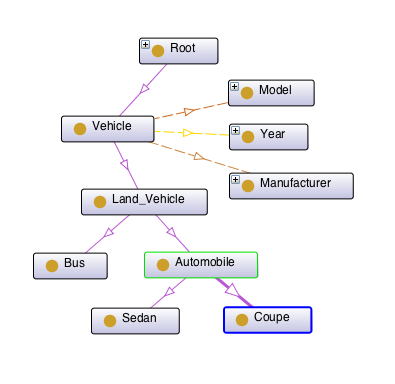
\includegraphics[scale=0.90]{OntologyDiagram.png}
	\caption{Abbreviated vehicular ontology}
	\label{fig:vehicular_ontology}
\end{figure}

\subsection{Executing} 

Once we have ranked the QRMs for a given user query, we can produce answers by re-visiting the pathways stored in the QRMs. The Morpheus \emph{Query Executor} (QE) evaluates a script of the query resolving process.  It simulates a human clicking buttons to follow links, submit forms, and highlight data, forming a textual answer.  The QE assumes that because of the auto generated nature of deep web pages, the location of answers are the same irrespective of page changes.  It uses the relative XPath location to the answer node on HTML pages as described in \cite{Badica06}.


